After implementing our system, the next step is conducting experiments. This will assist in evaluating and validating our thesis.
We focus on quantitative and qualitative results. To present our quantitative results we will use Average Precision at mean Intersection over Union (mIoU) thresholds of 
25\% and 50\% and for qualitative results will present a few of the point cloud segmentation and scene graphs generated using our system. 
For experiments, we have used the ARKITscenes dataset. They provide a large number of scenes enumerated by visit ID and each visit ID has at most three 
video recordings of the same scene denoted by video ID. For the purpose of experiments we divide the dataset into train, validation and test splits. We have trained
the Mask3D and PointNet models with a training set and validation set. Therefore, for experimentation, we will use the test split and evaluate the two SceneFun3D tasks defined 
earlier.
\begin{figure}[ht!]
    \centering
    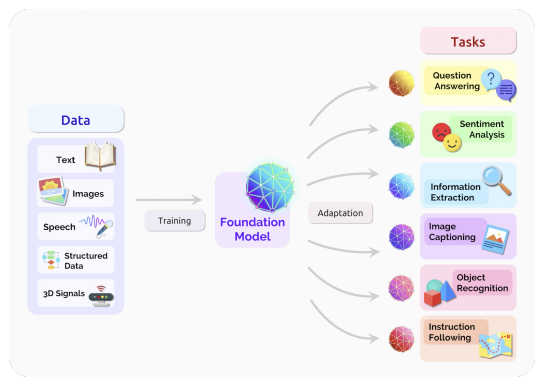
\includegraphics[width=0.8\textwidth]{images/FoundationModels.png}
    \caption{Scene graph of a scene from ARKITscenes (visit, video)}
    \label{fig:result1}
\end{figure}
\subsection{Scene graph generation on self captured dataset:}
One of the milestones of this thesis was to generate a scene graph using the dataset captured live, i.e. a real-world dataset. We performed experiments related to
 this task using two approaches. The first approach was to utilise the already recorded scenefun3D dataset which has real-world scenes. The second approach was 
to capture our dataset using the Intel Realsense camera in our own Socially Intelligent Robotics lab at the Institute of Artificial Intelligence, 
University of Stuttgart. We present the qualitative results for both of these approaches by showing some snaps of the final scene graphs generated 
using our system. \cref{fig:result1} is the scene graph for the scenefun3d dataset for video\_id\: and visit\_id\:. \cref{fig:result2} 
is the scene graph for our SIR lab.

\begin{figure}[ht!]
    \centering
    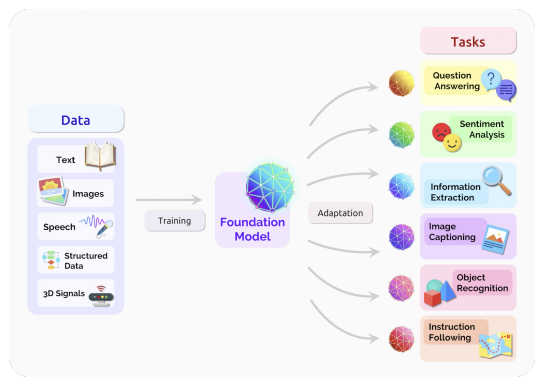
\includegraphics[width=0.8\textwidth]{images/FoundationModels.png}
    \caption{Scene graph of SIR lab.}
    \label{fig:result2}
\end{figure}
\subsection{Functionality segmentation:}
For this task, we will present both the quantitative results as well as the qualitative results. The results from scenefun3d for this task are taken as a baseline. 
SceneFun3D have adapted Mask3D for this task. They also compare SoftGroup and LERF. We have utilised Mask3D and PointNet ++ in our experiments. The reason for using 
Mask3D was to compare the results with scenefun3d and evaluate our method. PointNet ++ was leveraged as it is the state-of-the-art 3D CNN for part segmentation.

The table below compares the results from scenefun3d and our experiments. We also consider all the results from scenefun3d and do not only limit ourselves to
Mask3D. Additionally, we also include our point net ++ results.

\begin{longtable}{l|l|l|l}
    \caption{Quantitative result comparison for task functionality segmentation.} \label{tab:quantitativeResults} \\
    \hline \multicolumn{1}{|c|}{\textbf{Method}} & \multicolumn{1}{c|}{\textbf{AP}} & \multicolumn{1}{c|}{\textbf{AP\textsubscript{50}}} & \multicolumn{1}{c|}{\textbf{AP\textsubscript{25}}} \\ \hline
    SoftGroup-F & 3.6 & 17.2 & 11 \\
    LERF & 4.8 & 12.3 & 18.1\\
    Mask3D-F & 7.9 & 18.3 & 26.6\\
    Mask3D-Ours & 22.2 & 28.8 & 35.8\\
    PointNet & 22 & 22 & 22\\
    \hline
\end{longtable}
    
\begin{figure}[ht!]
    \centering
    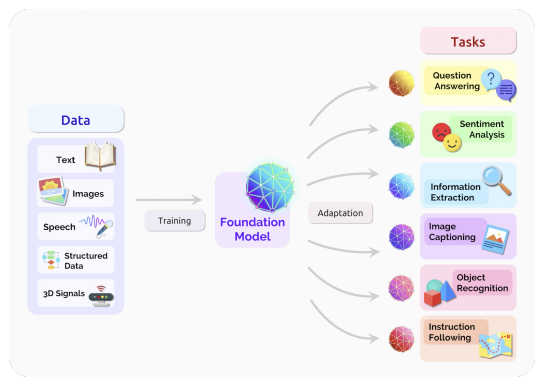
\includegraphics[width=0.8\textwidth]{images/FoundationModels.png}
    \caption{Part-Object segmentation results on ARKITscenes dataset.}
    \label{fig:task1result1}
\end{figure}
In addition to quantitative results, let us take a look at some qualitative results in \cref{fig:task1result1}. We compare our results with the ground truth.

\subsection{Task-driven affordance grounding:}
The results for this task will be presented as qualitative results with images from the output of our system. We query our concept graph with natural language
 and expect the system to return, the segmented point cloud as a heat map with the most probable object or part in a dark shade of red and 
 the least probable object or part in light blue. 

We ask our system two queries, \enquote{Open the cabinet below the mirror} and \enquote{Open the drawer of the cabinet next to the bathtub}. 
The results for the two queries are given below in \cref{fig:task2result1} and \cref{fig:task2result2}

\begin{figure}[ht!]
    \centering
    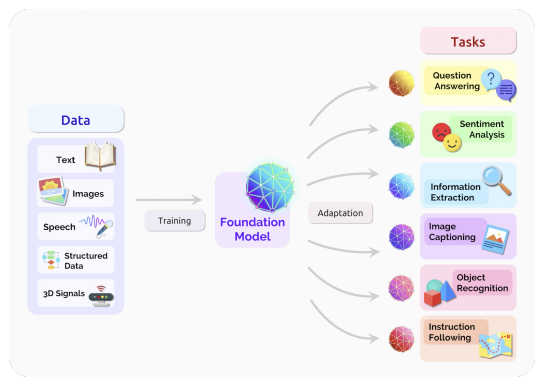
\includegraphics[width=0.8\textwidth]{images/FoundationModels.png}
    \caption{Qualitative result for Task-driven affordance grounding and query \enquote{Open the cabinet below the mirror}.}
    \label{fig:task2result1}
\end{figure}

\begin{figure}[ht!]
    \centering
    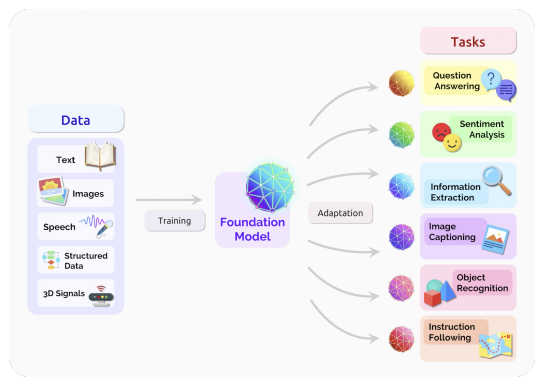
\includegraphics[width=0.8\textwidth]{images/FoundationModels.png}
    \caption{Qualitative result for Task-driven affordance grounding and query \enquote{Open the drawer of the cabinet next to the bathtub}.}
    \label{fig:task2result2}
\end{figure}